\documentclass[11pt,letterpaper]{article}
\usepackage[margin=1in]{geometry}
\usepackage{graphicx}
\usepackage{listings}
\usepackage{xcolor}
\usepackage{hyperref}
\usepackage{amsmath}
\usepackage{booktabs}
\usepackage{float}
\usepackage{caption}
\usepackage{subcaption}

% Code listing style
\lstset{
    language=C++,
    basicstyle=\ttfamily\small,
    keywordstyle=\color{blue}\bfseries,
    commentstyle=\color{gray}\itshape,
    stringstyle=\color{red},
    numbers=left,
    numberstyle=\tiny\color{gray},
    stepnumber=1,
    numbersep=5pt,
    backgroundcolor=\color{gray!10},
    frame=single,
    breaklines=true,
    captionpos=b,
    tabsize=4,
    showstringspaces=false
}

\title{ECE3849 Lab 1: FreeRTOS Stopwatch\\
\large Real-Time Embedded Systems}
\author{Benni Valentine \and Leo Riesenbach}
\date{\today}

\begin{document}

\maketitle

\section{Introduction}

In this lab we converted the bare-metal stopwatch from Lab 0 into a FreeRTOS-based application. Instead of a single \texttt{while(1)} loop, we now have four separate tasks handling timekeeping, buttons, display, and buzzer feedback. We also implemented a queue for communication between the button and buzzer tasks.

\section{System Architecture}

\begin{table}[H]
\centering
\caption{Task Configuration}
\begin{tabular}{lccl}
\toprule
\textbf{Task} & \textbf{Priority} & \textbf{Period} & \textbf{Responsibility} \\
\midrule
Time Task & 3 & 10 ms & Increment time counters \\
Button Task & 2 & 20 ms & Scan S1/S2, update state \\
Display Task & 1 & 33 ms & Render LCD \\
Buzzer Task & 1 & Event-driven & Process queue, drive PWM \\
\bottomrule
\end{tabular}
\end{table}

\begin{figure}[H]
    \centering
    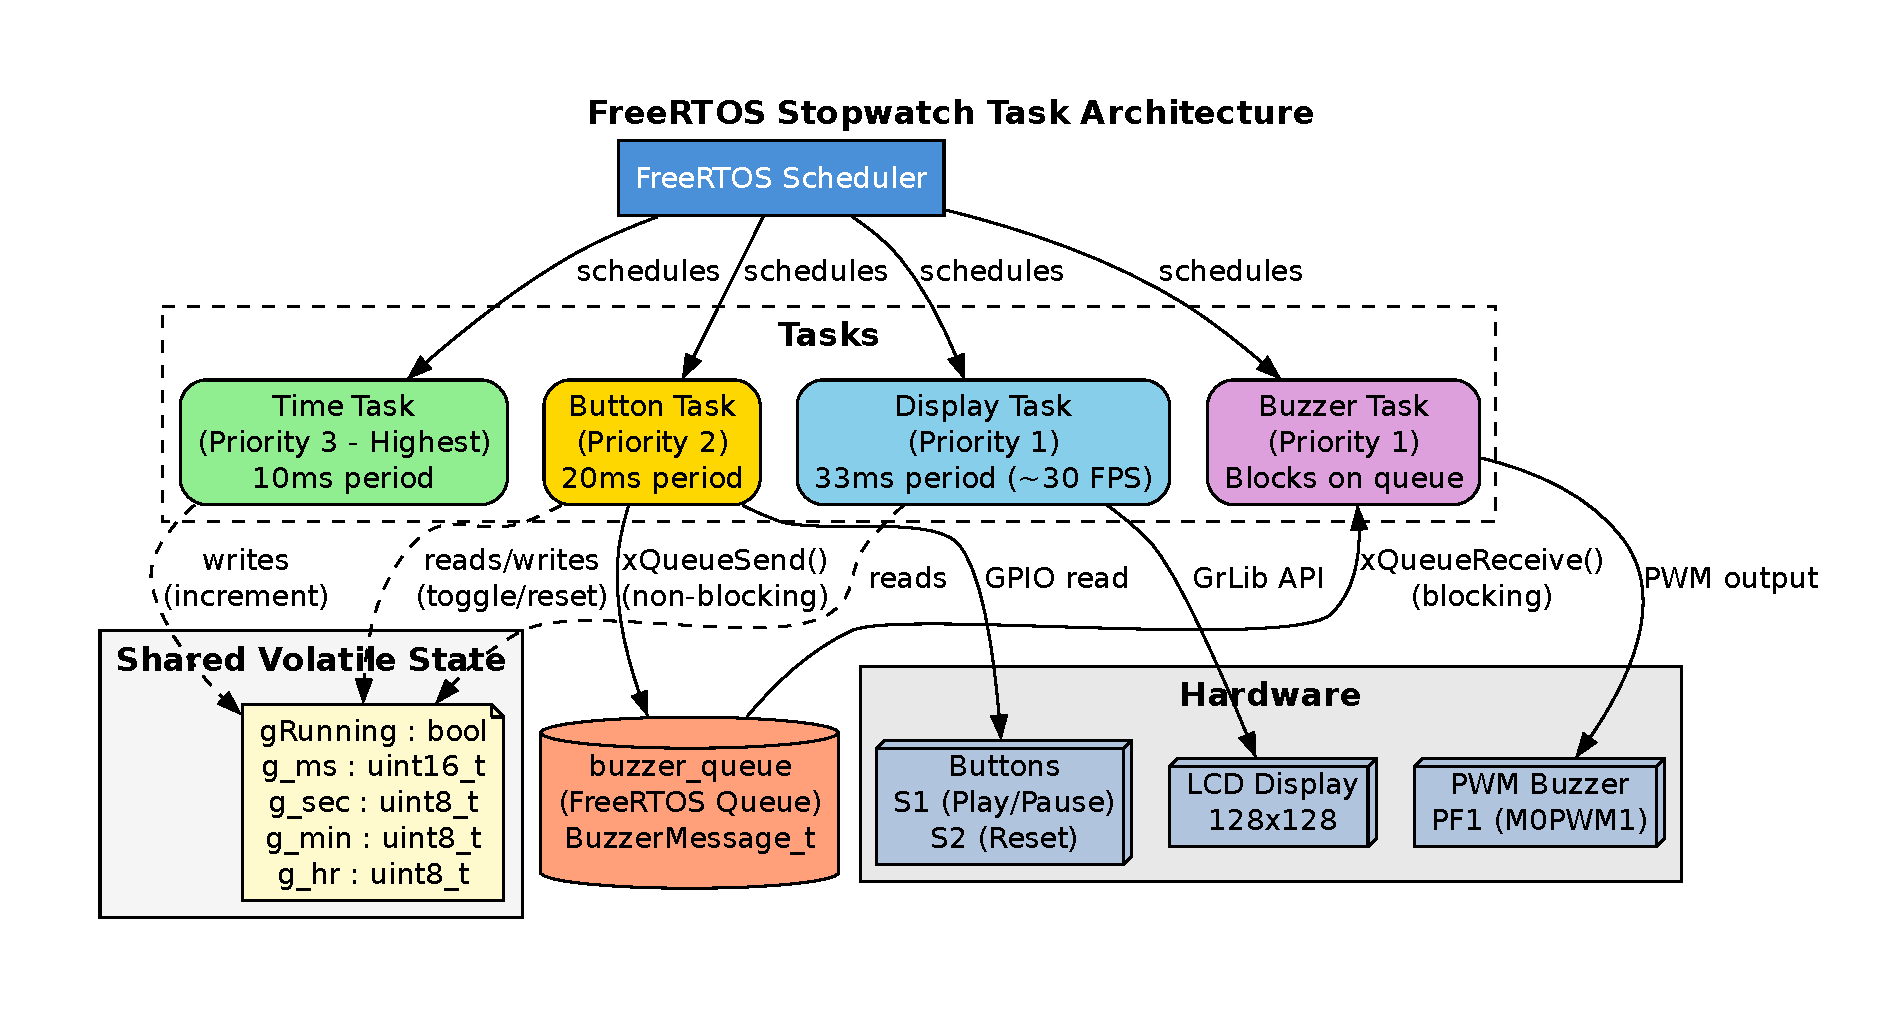
\includegraphics[width=0.95\textwidth]{diagrams/task_architecture.pdf}
    \caption{System Architecture}
    \label{fig:architecture}
\end{figure}

Time values are shared via \texttt{volatile} globals since only one task writes them. Buzzer commands use a queue so button presses can be buffered.

\section{Analysis Questions}

\subsection{Question 1: Role of port.c and portasm.asm}

\texttt{port.c} handles stack initialization, SysTick configuration, and critical sections, while \texttt{portasm.asm} contains the assembly routines for context switching (PendSV/SVC handlers). FreeRTOS needs processor-specific code because each architecture has different registers, stack layouts, and interrupt mechanisms that must be handled during task switching.

\subsection{Question 2: configTICK\_RATE\_HZ Analysis}

Our \texttt{configTICK\_RATE\_HZ} is set to 1000 Hz, so \texttt{vTaskDelay(pdMS\_TO\_TICKS(10))} equals 10 ticks. If set to 10 Hz, \texttt{pdMS\_TO\_TICKS(10)} would yield 0 ticks due to integer division, making 10 ms timing impossible.

\subsection{Question 3: Priority Assignment Rationale}

Time Task has the highest priority (3) since accurate timekeeping is critical, followed by Button Task (2) for responsive input, then Display and Buzzer Tasks (1) since they can tolerate delays. If Display had the highest priority and took 40 ms per frame, it would block the Time Task and cause the stopwatch to miss increments and run slow.

\subsection{Question 4: vTaskDelay vs. vTaskDelayUntil}

We used \texttt{vTaskDelayUntil()} for the timekeeping task. \texttt{vTaskDelay(n)} delays \texttt{n} ticks from when it's called, so execution time adds to the period. \texttt{vTaskDelayUntil()} delays until \texttt{n} ticks from the last wake time, keeping the period constant regardless of execution time, which prevents drift.

\subsection{Question 5: Button-to-Buzzer Data Flow}

Figure~\ref{fig:dataflow} shows the data flow from button press to buzzer sound.

\begin{figure}[H]
    \centering
    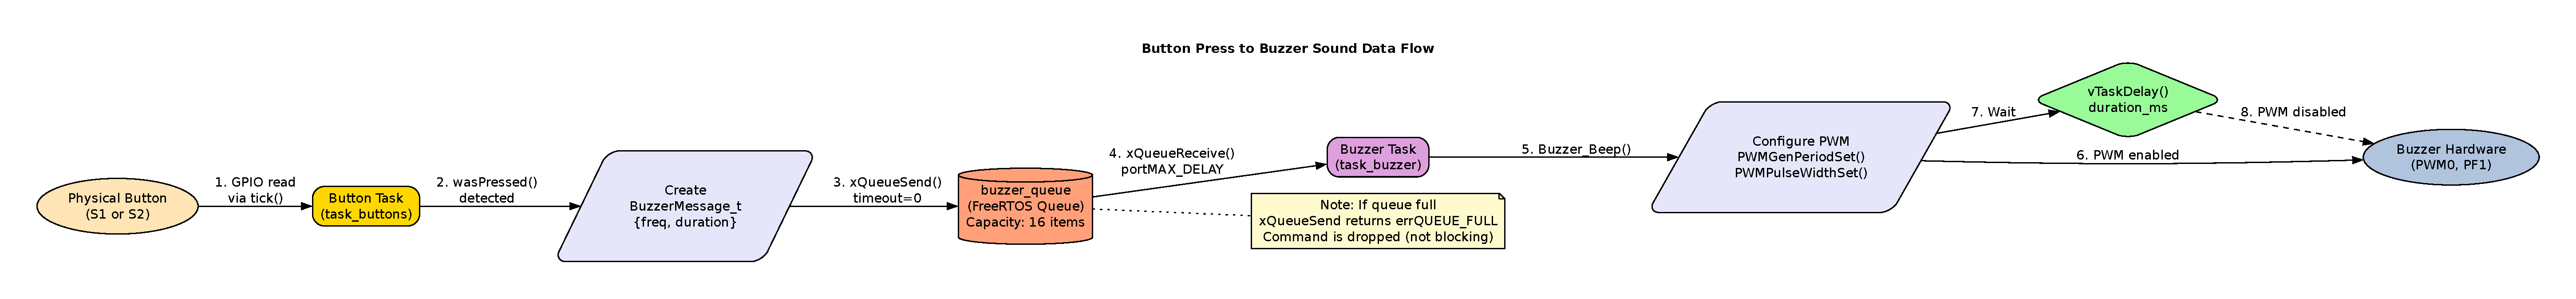
\includegraphics[width=0.95\textwidth]{diagrams/buzzer_dataflow.pdf}
    \caption{Button Press to Buzzer Sound Data Flow}
    \label{fig:dataflow}
\end{figure}

The Button Task detects a press, creates a \texttt{BuzzerMessage\_t} struct, and sends it via \texttt{xQueueSend()} with timeout 0. The Buzzer Task receives it with \texttt{xQueueReceive(portMAX\_DELAY)}, plays the tone using PWM, then blocks again. If the queue is full, the command is dropped and the button task continues without blocking.

\section{Debugging Challenges}

The most difficult part of this lab was debugging. The FreeRTOS system was essentially a black box, and when something didn't work, we had very limited visibility into what was happening internally.

We tried adding serial output via UART to print debug messages, but it didn't work properly with FreeRTOS. The UART calls would block and disrupt timing, output from multiple tasks would get garbled, and when hard faults occurred the UART would crash before printing anything useful. We also tried toggling LEDs at various points in the code, but tasks run too fast to see meaningful patterns.

Ultimately, we had to rely on careful code review and incremental development. We started with the basic LED blink test and added one task at a time, verifying each step worked before moving on. When we got unexplained crashes, increasing stack sizes usually fixed it.

\section{Conclusion}

The lab was completed successfully. Compared to Lab 0's bare-metal approach, the RTOS version has cleaner code organization with separate tasks, more accurate timing via \texttt{vTaskDelayUntil()}, and is easier to extend with new features. The trade-off is increased memory usage and more difficult debugging.

\end{document}
